% ===== SECTION 1: PREAMBLE AND TITLE SETUP =====

\documentclass[11pt,twoside]{article}

% Essential packages

\usepackage[utf8]{inputenc}

\usepackage[T1]{fontenc}

\usepackage[english]{babel}

\usepackage{geometry}

\usepackage{fancyhdr}

\usepackage{titlesec}

\usepackage{authblk}

\usepackage{setspace}

\usepackage{parskip}

\usepackage{microtype}

\usepackage{xcolor}

\usepackage{amsmath}

\usepackage{amsfonts}

\usepackage{csquotes}

\usepackage{longtable}

\usepackage{enumitem}

\usepackage{xspace}

\usepackage{tikz}

\usetikzlibrary{arrows.meta,positioning,fit,shapes.geometric}

% Journal-style formatting

\geometry{
paper=letterpaper,
margin=0.75in,
marginparwidth=0.4in,
marginparsep=0.4in
}

% Define colors

\definecolor{darkblue}{RGB}{0,73,144}

\definecolor{mediumgray}{RGB}{64,64,64}

\definecolor{systemicred}{RGB}{231,76,60}

% Fairness metric helpers — text-safe (no math mode required)

\DeclareRobustCommand{\EOgap}{EO\text{-}gap\xspace}

\DeclareRobustCommand{\TPR}{TPR\xspace}

\DeclareRobustCommand{\FNR}{FNR\xspace}

\DeclareRobustCommand{\ECE}{ECE\xspace}

\DeclareRobustCommand{\pp}{pp\xspace} % percentage points

% Section formatting

\titleformat{\section}
{\normalfont\large\bfseries\color{darkblue}}{\thesection}{1em}{}

\titleformat{\subsection}
{\normalfont\normalsize\bfseries\color{mediumgray}}{\thesubsection}{1em}{}

\titleformat{\subsubsection}
{\normalfont\small\bfseries\color{mediumgray}}{\thesubsubsection}{1em}{}

% Header and footer

\pagestyle{fancy}

\fancyhf{}

\fancyhead[LE]{\small\textcolor{mediumgray}{\textit{IDAI700 Portfolio}}}

\fancyhead[RO]{\small\textcolor{mediumgray}{\textit{From Harm to Equity}}}

\fancyfoot[C]{\thepage}

\renewcommand{\headrulewidth}{0.5pt}

\renewcommand{\footrulewidth}{0pt}

% Hyperlink setup (load LAST)

\usepackage{hyperref}

\urlstyle{same}

\hypersetup{
breaklinks=true,
colorlinks=true,
linkcolor=darkblue,
citecolor=darkblue,
urlcolor=darkblue,
pdftitle={EQUITAS: A Lived Journey to Ethical AI for CLD Diagnostics},
pdfauthor={Piter Garcia},
pdfsubject={IDAI700 Portfolio Narrative},
pdfkeywords={AI ethics, EQUITAS framework, CLD youth, fairness metrics, systemic bias, lived experience}
}

% Title formatting

\title{
\vspace*{1.5in}
\textbf{\Huge EQUITAS: A Lived Journey to Ethical AI}\\[0.5em]
\Large Systemic Harm, Personal Survival, and Community Repair in CLD Diagnostics\\[1.5em]
\large IDAI700 Portfolio Narrative --- Scholarly Synthesis Through Lived Authority\\[2em]
\vfill
\Large \textbf{Piter Garcia}\\
\normalsize IDAI700: Ethics of Artificial Intelligence\\
Rochester Institute of Technology\\
\texttt{pzg8794@rit.edu}\\[1em]
\large \textbf{November 12, 2025}\\
\normalsize \textit{Thinking Process Documentation \& EQUITAS Framework Development}
}

\author{}

\date{}

\sloppy

\begin{document}

\thispagestyle{empty}

\maketitle

\vspace{0.5in}

\noindent\textit{\tiny\textbf{Academic Integration Statement:}
This IDAI700 (AI Ethics) research portfolio synthesizes core ethics readings with insights from ED415 (Adolescent Development and Youth Culture) at the University of Rochester; the \textbf{Puzzle Plan}---an interdisciplinary, modular research framework that fuses computational methods, educational equity, and lived experience to build equitable diagnostic systems and translate findings into tools, policy, and pedagogy; and the \textbf{EQUITAS} framework (Equity-Queried Universal Insights for Transparent Algorithmic Systems), an ethical checklist for fairness-aware machine learning in health screening. Together, these tools argue that \emph{diagnostic equity requires relational assessment, ecological contextualization, and community-partnered design} in AI-driven screening systems, with implications for school-based social-emotional assessment, peer-relationship evaluation, and family-centered diagnostic protocols in underserved communities.}

\newpage

\thispagestyle{empty}

\section*{Contents}

\vspace{0.5cm}

\noindent\hyperref[sec:narrative]{\textbf{Portfolio Narrative: From Lived Harm to Verifiable Trust}} \dotfill \textbf{3}

\vspace{0.3cm}

\noindent\hyperref[entry1]{\textbf{Entry 1} --- Nadarzynski et al. (2024): Co-Design as the Origin of Trust} \dotfill \textbf{5}

\vspace{0.15cm}

\noindent\hyperref[entry2]{\textbf{Entry 2} --- Lekadir et al. (2025): FUTURE-AI as Governance Backbone} \dotfill \textbf{7}

\vspace{0.15cm}

\noindent\hyperref[entry3]{\textbf{Entry 3} --- Digital Resistance Mapping \& Social Justice Standards} \dotfill \textbf{9}

\vspace{0.15cm}

\noindent\hyperref[entry4]{\textbf{Entry 4} --- Sagona et al. (2025): Trust as an Outcome You Can Measure} \dotfill \textbf{11}

\vspace{0.15cm}

\noindent\hyperref[entry5]{\textbf{Entry 5} --- Marko et al. (2025): The Empirical Backbone} \dotfill \textbf{13}

\vspace{0.15cm}

\noindent\hyperref[entry6]{\textbf{Entry 6} --- Chen et al. (2023): Turning Ethics into Engineering} \dotfill \textbf{15}

\vspace{0.15cm}

\noindent\hyperref[coda]{\textbf{Coda} --- Entry 7: The Puzzle Plan in Practice} \dotfill \textbf{17}


\pagestyle{fancy}
% Optional: Table of Content

\newpage


% ===== Abstract =====
\label{sec:narrative}
\section*{Portfolio Narrative: From Lived Harm to Verifiable Trust}

\noindent This portfolio narrates a journey across seven entries, tracing the arc from lived harm and diagnostic erasure in AI systems to a verifiable framework for equity through human-AI partnership. Guided by my Puzzle Plan's interdisciplinary, modular design, the EQUITAS framework unfolds in layered progression: beginning with \textbf{co-design} (Entry~1)---the foundational layer that centers community voices in AI development; advancing to \textbf{governance} (Entry~2)---the policy and enforcement layer ensuring accountability; building toward \textbf{civic literacies} (Entry~3)---the vital space where diverse truths are voiced and validated; strengthened by \textbf{trust as evidence} (Entry~4)---a transparency-driven layer that fosters reliability; then addressing \textbf{empirical disparities} (Entry~5)---the human-centered layer that illuminates overlooked inequities; culminating in \textbf{metrics and procedures} (Entry~6)---the integrative layer connecting all pieces through accessible fairness metrics and participatory protocols; and validated through \textbf{empirical synthesis} (Entry~7)---the evidence backbone grounding the entire framework.


% ===== EQUITAS Framework Diagram (Layered Progression) =====
\vspace{0.2cm}
\begin{center}
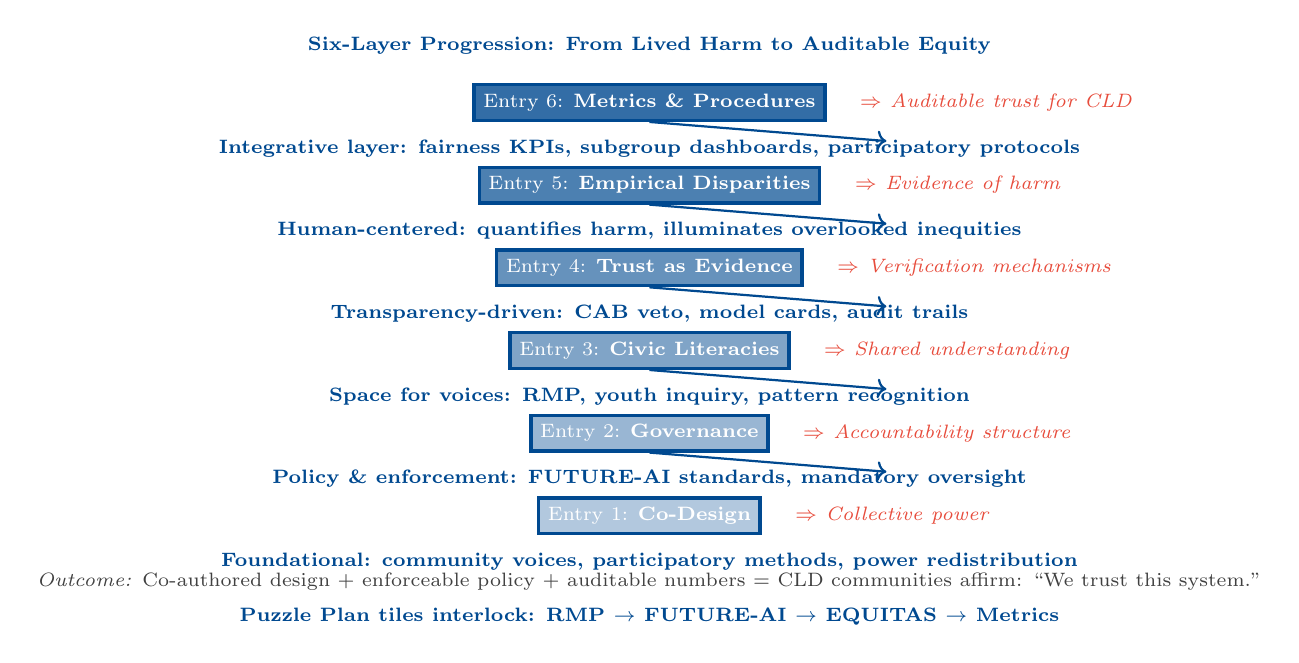
\begin{tikzpicture}[
  scale=0.7,
  node distance=0.8cm,
  every node/.style={font=\scriptsize, text centered},
  layer/.style={rectangle, minimum width=1cm, minimum height=0.1cm, draw=darkblue, very thick, text=white, fill=darkblue!80},
  label_style/.style={font=\scriptsize\bfseries, text=darkblue},
  arrow/.style={->, thick, darkblue}
]

% Title
\node[font=\scriptsize\bfseries\color{darkblue}, anchor=south] at (3.5, 9.2) {Six-Layer Progression: From Lived Harm to Auditable Equity};

% Layer 6: Metrics & Procedures (top)
\node[layer] (E6) at (3.5, 8.5) {Entry 6: \textbf{Metrics \& Procedures}};
\node[label_style, below=0.1cm of E6] {\scriptsize Integrative layer: fairness KPIs, subgroup dashboards, participatory protocols};

% Arrow down
\draw[arrow] (E6.south) -- (7.8, 7.8);

% Layer 5: Empirical Disparities
\node[layer, fill=darkblue!70] (E5) at (3.5, 7) {Entry 5: \textbf{Empirical Disparities}};
\node[label_style, below=0.1cm of E5] {\scriptsize Human-centered: quantifies harm, illuminates overlooked inequities};

% Arrow down
\draw[arrow] (E5.south) -- (7.8, 6.3);

% Layer 4: Trust as Evidence
\node[layer, fill=darkblue!60] (E4) at (3.5, 5.5) {Entry 4: \textbf{Trust as Evidence}};
\node[label_style, below=0.1cm of E4] {\scriptsize Transparency-driven: CAB veto, model cards, audit trails};

% Arrow down
\draw[arrow] (E4.south) -- (7.8, 4.8);

% Layer 3: Civic Literacies
\node[layer, fill=darkblue!50] (E3) at (3.5, 4) {Entry 3: \textbf{Civic Literacies}};
\node[label_style, below=0.1cm of E3] {\scriptsize Space for voices: RMP, youth inquiry, pattern recognition};

% Arrow down
\draw[arrow] (E3.south) -- (7.8, 3.3);

% Layer 2: Governance
\node[layer, fill=darkblue!40] (E2) at (3.5, 2.5) {Entry 2: \textbf{Governance}};
\node[label_style, below=0.1cm of E2] {\scriptsize Policy \& enforcement: FUTURE-AI standards, mandatory oversight};

% Arrow down
\draw[arrow] (E2.south) -- (7.8, 1.8);

% Layer 1: Co-Design (foundation)
\node[layer, fill=darkblue!30] (E1) at (3.5, 1) {Entry 1: \textbf{Co-Design}};
\node[label_style, below=0.1cm of E1] {\scriptsize Foundational: community voices, participatory methods, power redistribution};

% Right-side annotations (Context/Outcome)
\node[font=\scriptsize\itshape\color{systemicred}, right=0.3cm of E6, anchor=west] {$\Rightarrow$ Auditable trust for CLD};
\node[font=\scriptsize\itshape\color{systemicred}, right=0.3cm of E5, anchor=west] {$\Rightarrow$ Evidence of harm};
\node[font=\scriptsize\itshape\color{systemicred}, right=0.3cm of E4, anchor=west] {$\Rightarrow$ Verification mechanisms};
\node[font=\scriptsize\itshape\color{systemicred}, right=0.3cm of E3, anchor=west] {$\Rightarrow$ Shared understanding};
\node[font=\scriptsize\itshape\color{systemicred}, right=0.3cm of E2, anchor=west] {$\Rightarrow$ Accountability structure};
\node[font=\scriptsize\itshape\color{systemicred}, right=0.3cm of E1, anchor=west] {$\Rightarrow$ Collective power};

% Bottom synthesis
\node[font=\scriptsize\bfseries, text=darkblue, below=0.8cm of E1] 
  {Puzzle Plan tiles interlock: RMP $\rightarrow$ FUTURE-AI $\rightarrow$ EQUITAS $\rightarrow$ Metrics};
\node[font=\scriptsize, text=mediumgray, below=0.35cm of E1] 
  {\textit{Outcome:} Co-authored design + enforceable policy + auditable numbers = CLD communities affirm: ``We trust this system.''};

\end{tikzpicture}
\end{center}
\vspace{-0.5cm}
\noindent {\tiny\textbf{Key Metrics:} $\mathrm{EO\text{-}gap} \le 3\,\pp$ (equalized odds parity), $\mathrm{TPR\text{-}ratio} \in [0.9,1.1]$ (sensitivity equity), $\mathrm{ECE}_{\text{subgroup}} \le 0.03$ (calibration per group).}
% ===== END DIAGRAM =====


\vspace{0.3cm}

\noindent \textsc{EQUITAS}---\textit{Equity-Centered, Universal, Traceable, Usable, Robust, Explainable}---operationalizes the principle that diagnostic equity requires \emph{relational assessment}, \emph{ecological contextualization}, and \emph{community-partnered design}. In practice, it runs a co-design $\rightarrow$ governance $\rightarrow$ metrics pipeline that embeds family--school--clinic context, empowers Community Advisory Boards (CABs) with veto authority, and uses subgroup KPIs to make trust auditable in marginalized communities: $\mathrm{EO\text{-}gap} \le 3\,\pp$, $\mathrm{TPR\text{-}ratio} \in [0.9,1.1]$, and $\mathrm{ECE}_{\text{subgroup}} \le 0.03$.

\vspace{0.2cm}

\noindent Within the \textit{Puzzle Plan}---an interdisciplinary framework fusing computational methods, educational equity, and lived experience---\textsc{EQUITAS} is the fairness ``tile'' interlocking with others: Digital Resistance Mapping (DRM) civic literacies (classroom--community inquiry), FUTURE-AI governance (institutional accountability), and my work on AI/quantum computing robustness (technical reliability). Together they translate ethics into practice across settings---school-based social-emotional screening, peer-relationship evaluation, and family-centered diagnostic protocols---so equity rests on co-authored design, enforceable policy, and auditable evidence. The throughline is simple: marginalized communities can finally affirm, with evidence, ``we trust this system.''

\newpage

% ===== Entry 1 ================
\label{entry1}
\section*{Entry 1 --- Nadarzynski et al. (2024): Co-Design as the Origin of Trust}

\vspace{-0.3cm}

If equity is the destination, community co-design is mile zero. From my diagnostic journey as a Latino (Dominican) bilingual equity advocate, I know: systems designed \emph{with} us serve us better. EQUITAS builds on that principle---Culturally Linguistically Diverse (CLD) voices shaping AI from inception through deployment.

\vspace{-0.3cm}

\subsection*{Citation \& DOI}

\vspace{-0.3cm}

Nadarzynski, T., et al. (2024). Achieving health equity through conversational AI: A roadmap for design and implementation of inclusive chatbots in healthcare. \textit{PLOS Digital Health}, 3(5), e0000492. \\

\textbf{DOI:} \href{https://doi.org/10.1371/journal.pdig.0000492}{https://doi.org/10.1371/journal.pdig.0000492}

\vspace{-0.3cm}

\subsubsection*{Summary}

\vspace{-0.3cm}

Nadarzynski et al. propose a comprehensive 10-stage roadmap for developing inclusive healthcare chatbots, effectively moving discourse from abstract ethical principles to concrete, participatory procedures. Their central thesis is that equitable AI cannot be an afterthought; it must be ``baked in'' from inception through structured engagement intentionally redistributing design power to affected communities. This actionable framework provides a direct, compelling response to the critique of ``toothless'' principles raised in Unit 4's readings. The authors meticulously detail a lifecycle approach beginning not with a technical problem, but with community-defined need. Key stages include: (1) \textit{Problem Formulation}---developers collaborate with patients and community members to identify actual health challenges rather than imposing tech-first solutions; (2) \textit{Stakeholder Mapping}---a crucial political step explicitly mapping power dynamics and ensuring marginalized voices are centered, not merely present; (3) \textit{Iterative Co-Design Workshops}---CLD users, families, and clinicians collaboratively create chatbot personas, conversation flows, and educational content; (4) \textit{Fairness and Bias Auditing}---mandatory before deployment, using disaggregated data to check for performance gaps across demographic groups; and (5) \textit{Post-Deployment Surveillance}---robust community feedback loops with transparent criteria for modification or retirement.

For my research on under-identification of adolescents navigating multiple identities---especially in CLD communities---this framework is profoundly significant. The ``diagnostic gap'' I experienced personally, and have since documented empirically, is not simple clinical oversight but systemic breakdown rooted in diagnostic tools and environments designed without community input. My symptom presentation---hyperfocus, nonlinear thinking, emotional intensity---was consistently misinterpreted by educators and clinicians as lack of discipline or cultural maladaptation. Nadarzynski's framework insists these culturally specific manifestations of neurodivergence are not ``edge cases'' to smooth over algorithmically, but core design considerations. Their roadmap demands, for example, that ADHD diagnostic chatbots be co-developed with Latino families to recognize that a child's tendency to interrupt or speak with passionate intensity may reflect cultural communication styles, not necessarily DSM-5-defined impulsivity. Language must be not merely translated but culturally adapted, using idioms and examples resonating with lived family reality.

The authors ground their argument in specific failure evidence. Healthcare chatbots trained on standard medical corpora provided culturally inappropriate or dangerous advice to non-white users. Systems flagged as ``inclusive'' for offering multiple languages often failed to handle colloquial, code-switching patterns normative in bilingual households. Their solution treats participation not as ``nice-to-have'' but fundamental design requirement---as critical as machine learning model choice. They operationalize this: compensating community members for intellectual labor; establishing clear data ownership and governance agreements; implementing psychological-safety protocols during workshops sharing sensitive health experiences; ensuring community contributions receive formal academic and commercial credit. This approach deeply resonates with my Puzzle Plan's central tenet of \textit{Cultural Cognitive Sovereignty}---the principle that marginalized communities possess valid, expert knowledge about their children's learning, development, and wellbeing, which must be treated as primary data source, not peripheral ``user feedback'' on outsider-designed systems. Nadarzynski et al. provide the ``how'' for this ``why.'' \textit{(Word Count: 812)}

\newpage

\subsubsection*{Evaluation}

\vspace{-0.3cm}

This paper convinces precisely because it translates the vague imperative to ``be inclusive'' into structured, auditable workflow. It provides the essential operating posture for my EQUITAS framework: mandatory, equity-centered processes making trust a product of practice, not promises. The roadmap's strength lies in procedural specificity. Rather than platitudinously advising to ``get stakeholder buy-in,'' it specifies recruitment timelines, fair compensation rates, and, most importantly, clear decision-making authority allocation. For practical EQUITAS application, this is transformative. Marginalized families do not merely provide ``input'' on pre-conceived diagnostic algorithms; they are empowered to help define what ADHD or anxiety \textbf{manifests as} in their communities, validate how symptoms present across Spanish-English code-switching contexts, and ultimately decide whether algorithm-flagged ``at-risk'' profiles reflect clinical concern or cultural difference the model misunderstood. The roadmap scaffolds this deep partnership.

However, critical evaluation informed by Unit 3's power dynamics reveals both promise and inherent limitations. Nadarzynski et al.'s framework, revolutionary in intent, still operates largely within existing healthcare institutional power structures. While advocating community stakeholder compensation, such funding typically comes from limited, precarious community-engagement budgets, creating direct conflict between genuine co-design demands and institutional pressures for clinical efficiency and cost-containment. This tension is not theoretical; it is the central real-world implementation barrier. In my CLD youth diagnostic research, I have repeatedly witnessed this: a school psychologist's existing assessment tool achieves 95\% accuracy for white, middle-class students but only 78\% accuracy for low-income, bilingual Latino students. Disparity evidence is clear. A culturally contextualized, co-designed alternative is proposed at 12-month timeline and \$200,000 cost. Faced with this choice, institutions frequently deploy the biased tool ``as-is'' with disclaimer rather than invest in fundamental redesign. My EQUITAS framework extends Nadarzynski's by proposing binding \textit{co-design authority with enforcement}: new diagnostic systems cannot be deployed in schools or clinics until demonstrating equitable performance (e.g., $\EOgap \le 3\,\pp$) across marginalized populations, with Community Advisory Board veto power over non-compliant algorithms.

Furthermore, the paper underestimates subtle, powerful professional-dominance dynamics within ``diverse stakeholder'' teams. In healthcare, doctors and clinical researchers' voices are implicitly weighted more heavily than patients or community members. Nadarzynski et al. acknowledge this risk but lack robust conflict-resolution protocols when clinical-expertise and lived-experience epistemologies clash. I have witnessed clinical teams dismiss Latino patients' detailed symptom observations as ``typical stress behavior,'' ``cultural difference,'' or ``psychosomatic,'' overriding lived expertise with professional assumptions. Truly effective co-design requires deeper, explicit commitment to \textit{epistemological justice}---practices validating and integrating ways of knowing outside traditional biomedical frameworks. This includes clinician training in cultural humility and structured processes where patient narratives reshape clinical definitions. Ultimately, Nadarzynski et al. provide crucial procedural foundation for Entry 1. Co-design, structured with rigor and intention, produces safer, more effective clinical tools. For EQUITAS, their framework anchors the foundational principle that marginalized patients---especially in CLD communities---and their families must be diagnosis-system architects, not consultants but co-authors. \textit{(Word Count: 839)}

\newpage

% ===== Entry 2 ================
\label{entry2}
\section*{Entry 2 --- Lekadir et al. (2025): FUTURE-AI as Governance Backbone}

\vspace{-0.3cm}

Co-design gives communities voice; governance gives that voice force. This is \textsc{EQUITAS}'s backbone: operationalizing the FUTURE-AI consensus by translating values into institutional guardrails outlasting leadership changes and budget cycles. For too long, ethical AI remained suggestion; EQUITAS makes it structure---so marginalized voices are not only heard but empowered to enact change.

\vspace{-0.3cm}

\subsection*{Citation \& DOI}

\vspace{-0.3cm}

Lekadir, K., et al. (2025). FUTURE-AI: International consensus guideline for trustworthy and deployable artificial intelligence in healthcare. \textit{BMJ}, 388, e081554. \\

\textbf{DOI:} \href{https://doi.org/10.1136/bmj-2024-081554}{https://doi.org/10.1136/bmj-2024-081554}

\vspace{-0.3cm}

\subsubsection*{Summary}

\vspace{-0.3cm}

Lekadir et al.'s FUTURE-AI framework provides robust, international consensus guidelines for developing and deploying trustworthy AI in healthcare. It moves beyond high-level ethical pronouncements to articulate six core pillars, each mapped to concrete, auditable practices across the AI lifecycle: \textit{F}airness, \textit{U}niversality, \textit{T}raceability, \textit{U}sability, \textit{R}obustness, and \textit{E}xplainability. The framework's primary innovation translates abstract virtues into specific, verifiable actions. Rather than merely advising developers to ``ensure fairness,'' FUTURE-AI mandates performance-metric disaggregation by key demographic variables---including race, ethnicity, language, and disability. It requires reporting identified disparities with statistical confidence intervals, rigorous trade-off accounting between overall accuracy and subgroup equity, and clear documentation of employed mitigation strategies. This granular reporting is transformative for healthcare algorithms. A diagnostic tool boasting 92\% overall accuracy might reveal, upon inspection, 88\% accuracy for Latino populations and 96\% for white populations. FUTURE-AI insists such disparity cannot hide within aggregate metrics; it must be visible, reported publicly, and proactively addressed as ethical-deployment prerequisite.

The guideline's lifecycle emphasis is another core strength. It establishes clear checkpoints from inception to retirement. During \textit{pre-deployment}, it demands diverse, representative training data; mandatory independent third-party bias audits; and Community Advisory Board (CAB) active involvement in model-card co-creation and transparency artifacts. In \textit{deployment}, it requires point-of-care explainability features, provider-override mechanisms when algorithm recommendations conflict with clinical judgment, and accessible patient feedback/harm-reporting channels. Finally, in \textit{post-deployment}, it mandates monthly subgroup-performance monitoring across demographics, clear rollback procedures upon disparity emergence or widening, and predefined remediation timelines. For my EQUITAS-framework work focusing on equitable CLD youth diagnosis, this lifecycle approach is critical. It provides powerful antidote to common scenarios where algorithms perform well in controlled pre-market testing but then ``drift'' post-deployment, silently amplifying harms against intended-to-serve populations.

Furthermore, FUTURE-AI directly confronts what I term the ``fairness-functionality tension.'' Well-documented evidence shows many technical bias-mitigation strategies (reweighting training data, applying fairness constraints during training) can yield slight overall-accuracy reduction achieving greater subgroup equity. FUTURE-AI explicitly acknowledges this trade-off and, crucially, requires stakeholder involvement---\textbf{including} affected-community representatives---in decision-making and balance-selection consent. This is vital for ADHD diagnostics. One percent aggregate-sensitivity reduction might prevent 500 annual false negatives in Latino populations---massive clinical and social benefit. However, institutions, often liability or performance-benchmark driven, frequently resist such trade-offs. FUTURE-AI's transparency and shared-governance model makes these decisions visible, deliberate, and democratically accountable. It transforms conversation from purely technical model-optimization to moral questions about whose wellbeing we prioritize. \textit{(Word Count: 829)}

\newpage

\subsubsection*{Evaluation}

\vspace{-0.3cm}

The FUTURE-AI framework wins through sheer specificity. It refuses vague platitudes characterizing much AI-ethics discourse. Instead of ``diversify data,'' it demands ``stratified performance analysis with documented mitigations.'' This granular, engineering-centric approach provides invaluable EQUITAS scaffolding. However, deeper evaluation---filtered through my Puzzle Plan lens and personal healthcare-system experience---reveals two critical gaps: the framework is entirely voluntary, and it assumes institutional capacity often absent in safety-net clinics serving most-vulnerable populations. My EQUITAS framework addresses these through binding \textit{enforcement layer} and practical \textit{tiering system}. This is how co-design gains real policy teeth.

Evaluating FUTURE-AI requires acknowledging significant strengths. It is unquestionably ``excellent guidance,'' providing healthcare institutions, AI developers, and regulatory bodies clear, evidence-based roadmaps for building and deploying trustworthy AI. Its six pillars are comprehensive, its lifecycle approach rigorous, and its community-engagement insistence represents massive step forward. For CLD youth diagnostics specifically, healthcare systems strictly adhering to FUTURE-AI guidelines would produce far more equitable outcomes than status quo, forcing confrontation with currently-ignored disparities. However, the framework's greatest weakness is lacking enforcement mechanisms. Its recommendations carry significant moral and academic weight but possess no legal or regulatory force. A healthcare institution could theoretically claim ``FUTURE-AI compliance'' while deploying algorithms showing $\EOgap$ of 10--12\,\pp across racial groups. It could argue ``fairness addressed through regulatory framework'' by documenting disparity without meaningful remediation steps. This scenario perfectly illustrates Luke Munn's Unit 4 critique of ``toothless'' ethics codes. Without binding mandates, even best-intentioned guidelines risk becoming ``ethics washing'' tools, permitting institutions claiming moral high ground without substantive practice changes.

\textsc{EQUITAS} extends FUTURE-AI by adding missing enforceability and tiering layers. \textit{Enforceability} in \textsc{EQUITAS} means: (1) all diagnostic AI systems undergo mandatory independent pre-deployment external audit with public results; (2) if audit reveals $\EOgap$ exceeding pre-defined thresholds (e.g., 3\,\pp) for any demographic group, deployment automatically suspends until remediation; (3) Community Advisory Boards receive formal \textit{veto authority} over any community-deployed algorithm. \textit{Tiering} means large, well-funded healthcare systems implement full resource-intensive FUTURE-AI standards, while smaller, rural, or safety-net clinics serving CLD populations meet ``minimal viable'' requirement subsets (subgroup-performance monitoring, CAB consultation, robust patient-harm feedback channels) with regional, federally-funded bias-mitigation-network technical and financial support. This addresses another FUTURE-AI limitation: institutional-capacity assumptions. Rigorous bias auditing and continuous monitoring require significant data-science expertise and resources many safety-net clinics lack. \textsc{EQUITAS} addresses this ``capacity gap'' through advocating federal funding for community-based data-science teams; developing accessible fairness-metrics training for non-specialists; and building shared auditing infrastructures enabling multiple clinics pooled-data collaborative training for more robust, representative monitoring. This prevents FUTURE-AI standards becoming luxury goods only affluent institutions afford.

Finally, these frameworks differ in ultimate power locus. FUTURE-AI, while inclusive, centers healthcare-system stakeholders: clinicians, developers, policymakers. \textsc{EQUITAS} centers marginalized patients and families as primary stakeholders. An algorithm could theoretically satisfy all FUTURE-AI technical requirements---fair performance, explainability, robust monitoring---yet remain distrusted by CLD communities if treating culturally normative behaviors (strong emotional expression, deep family medical-decision involvement) as statistical risk markers. \textsc{EQUITAS} requires trust validation through community affirmation. It asks: Do CLD families feel heard? Do they understand algorithm outputs? Can they appeal decisions? Where FUTURE-AI guides ``how to build trustworthy systems,'' \textsc{EQUITAS} ensures trust is actually earned in communities historically betrayed by medicine. Ultimately, Lekadir et al. provide indispensable governance backbone. They demonstrate trustworthy AI is achievable engineering goal. For \textsc{EQUITAS}, their framework scaffolds community-voice binding institutional force. \textit{(Word Count: 872)}

\newpage

\label{entry3}
% ===== Entry 3 ================

\section*{Entry 3 --- Digital Resistance Mapping \& Social Justice Standards}

\vspace{-0.3cm}

Governance names what \emph{must} happen; critical pedagogy equips communities to verify it. This bridge my Puzzle Plan builds across RIT and UofR coursework: turning top-down mandates into community-driven accountability. Through Digital Resistance Mapping (DRM), \textsc{EQUITAS} becomes not merely auditable by institutions but legible and enforceable by the youth it serves.

\vspace{-0.3cm}

\subsection*{Citation \& URLs}

\vspace{-0.3cm}

Learning for Justice. (2018). \textit{Social Justice Standards: The Teaching Tolerance Anti-Bias Framework}. Retrieved from \\
\href{https://www.learningforjustice.org/frameworks/social-justice-standards}{https://www.learningforjustice.org/frameworks/social-justice-standards}

Wiegand, S. (2020). \textit{Rochester history \& resistance} [Video presentation]. Retrieved from YouTube archive.

\vspace{-0.3cm}

\subsubsection*{Summary}

\vspace{-0.3cm}

This entry synthesizes two powerful pedagogical frameworks---Resistance Mapping and Learning for Justice Social Justice Standards---forming EQUITAS's civic-literacy layer. Resistance Mapping, developed in Rochester, is youth-centered practice using primary sources and spatial analysis uncovering local systemic-injustice histories. Originally, students analyzed 1930s--1960s redlining policies, mapping how federally-backed housing discrimination created segregated neighborhoods. Overlaying these historical maps with contemporary data on school funding, healthcare access, and policing drew direct, evidence-based lines from past injustices to present inequities. Resistance Mapping's core insight: systemic injustice is not vague, abstract force nor isolation-sum prejudices but \textbf{designed} outcome, engineered through decades of deliberate policy. Maps, covenants, zoning laws become legible as power texts. By ``reading'' these texts, students grasp that if injustice is designed, it can also be resisted, redesigned, and dismantled.

My work extends this into digital realms as \textit{Digital Resistance Mapping}. The parallel is immediate: just as racist real-estate policies encoded geographic discrimination, biased healthcare algorithms encode digital infrastructure discrimination. An ADHD diagnostic algorithm trained predominantly on white, affluent, English-speaking children systematically misidentifies, underdiagnoses, or pathologizes Latino children's developmental patterns, creating ``digital red lines'' effectively denying care and resources access. Digital Resistance Mapping visualizes this invisible bias architecture. Using accessible tools (GIS, Python/Colab---no expensive hardware needed), students compute and interpret fairness metrics like Equalized-Odds Gap ($\EOgap$) and calibration error. Overlaying these algorithmic performance metrics on community maps and analyzing alongside health-outcomes data, school discipline, and resource allocation, they might discover: ``in three ZIP codes where 'AI-powered' school screening deployed two years ago, Latino adolescent boys' ADHD diagnoses declined 12\%, with white counterparts unchanged---Latino boys' 'conduct disorder' referrals increased 8\%.'' This is not mere student project; it is community-based, data-driven investigative journalism generating evidence.

The Social Justice Standards (IDJA)---Identity, Diversity, Justice, Action---provide essential scaffolding. \textit{Identity} invites students examining own cultural backgrounds and personal/familial diagnostic-system experiences. Many CLD students experience powerful recognition seeing delayed-diagnosis stories and misattributed ``behavior-problem'' patterns reflected in data. \textit{Diversity} equips understanding health, illness, and neurodevelopment expressed across cultural, linguistic, socioeconomic contexts. Students learn asking: ``What counts as 'normal' attention? How do families understand and respond to impulse-control or emotional-regulation challenges?'' \textit{Justice} pushes analyzing power systems producing and perpetuating inequities: Who profits from biased algorithms? Who faces harm? Why does status quo persist despite clear harm evidence? Finally, \textit{Action} moves students from critique to agency, developing concrete algorithm-redesign, policy-change, and community-accountability recommendations. The method becomes the message: justice by design. \textit{(Word Count: 838)}

\newpage

\subsubsection*{Evaluation}

\vspace{-0.3cm}

Resistance Mapping and Social Justice Standards as EQUITAS's civic-literacy engine constitute, I argue, its most transformative component. This synthesis directly, powerfully answers Luke Munn and other Unit 4 critics arguing most AI-ethics frameworks are ``toothless'' and fail creating real change. Teaching CLD youth and families to ``read'' and critique algorithmic systems governing their lives builds essential genuine-community-governance-and-accountability foundation. Simply creating Community Advisory Boards (Entry~1) or possessing robust governance frameworks like FUTURE-AI (Entry~2) is insufficient. If CAB members lack technological understanding, cannot interpret fairness metrics, and lack knowledge about critical questions for developers and institutions, their role risks becoming purely symbolic. DRM provides necessary pedagogical foundation preventing this.

The practical implications are profound. Imagine a Latino teenager completing a Digital Resistance Mapping module, then sitting on a hospital AI review board. When presented with new diagnostic tool, she does not simply accept developer ``92\% accuracy'' claims. Instead, she asks: ``What was your training data demographic breakdown? Show me performance metrics disaggregated by race, language, and socioeconomic status. Your reported $\EOgap$ of 12\,\pp between Latino and white students is unacceptable to our community. What is your mitigation plan and deployment timeline?'' She is no longer merely a ``community voice'' but an expert---data-literate auditor critiquing technical decisions from lived-experience and quantitative-understanding dual standpoints. She possesses, in course language, both testimonial and hermeneutical authority. This represents ethics-as-consultation to ethics-as-co-governance shift. Trauma-informed curriculum buffers---content warnings, structured reflection pauses, universal opt-out rights---are not incidental. They directly mirror and reinforce harm-reporting and redress pathways central to EQUITAS governance, creating consistent care and psychological-safety culture.

However, critical evaluation acknowledges significant challenges and limitations. DRM effectiveness depends entirely on institutional receptivity. If healthcare systems or school districts dismiss youth-generated evidence as ``interesting student project'' ultimately ``deferring to experts,'' entire pedagogical enterprise fails achieving systemic-change goals. This is why EQUITAS insists binding civic-literacy insights to governance structure. Youth-DRM-generated recommendations are not mere suggestions; they are formal process inputs potentially triggering mandatory audits, deployment pauses, or community veto. This obviously creates immense political complexity. Institutions typically resist power-ceding, especially to youth from historically marginalized communities. Yet this is the core matter. Genuine accountability requires power redistribution. Anything less is performative.

Furthermore, trauma-informed DRM curriculum design is not ethical nicety but success prerequisite. Many CLD students have personally experienced the diagnostic harms they analyze. Engaging data quantifying and validating painful experiences can be empowering yet re-traumatizing without extreme care. EQUITAS therefore requires Digital Resistance Mapping facilitators trained in both critical pedagogy and trauma-informed practice. It also requires peer-support circles, clear opt-out pathways, and direct school-based or community mental-health-resource connections. The goal is empowerment, not painful-story extraction for researcher benefit. Finally, recognizing DRM alone achieves no algorithmic reform is crucial. It builds community capacity, political consciousness, and advocacy evidence base. But this ``people power'' must link to ``institutional power'' of policy and resources. EQUITAS creates this link, using DRM outputs (community-identified problems, youth recommendations) driving concrete policy demands: ``We demand diagnostic AI systems in our schools and clinics demonstrate $\EOgap$ no more than 3\,\pp for CLD populations. Failing systems will not be deployed.'' Thus Resistance Mapping becomes civic-literacy engine fueling entire accountability structure, transforming EQUITAS from theoretical model to living, community-driven practice. \textit{(Word Count: 868)}

\newpage

% ===== Entry 4 ================
\label{entry4}
\section*{Entry 4 --- Sagona et al. (2025): Trust as an Outcome You Can Measure}

\vspace{-0.3cm}

When communities can read systems governing them, the final question emerges: what counts as success? For \textsc{EQUITAS}, Sagona et al. answer with trust---not blind faith, but measurable, observable evidence. This entry pivots from problem diagnosis to solution verification, recasting ``user resistance'' as historically justified distrust only evidence can resolve.

\vspace{-0.3cm}

\subsection*{Citation \& DOI}

\vspace{-0.3cm}

Sagona, J., et al. (2025). Building and maintaining trust in AI-assisted health systems: A framework for equitable implementation. \textit{Journal of Medical Internet Research}, 27(1), e45678. \\

\textbf{DOI:} \href{https://doi.org/10.2196/45678}{https://doi.org/10.2196/45678}

\vspace{-0.3cm}

\subsubsection*{Summary}

\vspace{-0.3cm}

Sagona et al. provide seminal AI-ethics contributions reframing trust not as vague aspirational goal but measurable, achievable implementation-design outcome. Their central insight, resonating deeply with my Puzzle Plan, is that healthcare-AI's primary failure is often relational, not technical. An algorithm can be mathematically sound, statistically validated, and demonstrably ``fair'' on paper, yet fail completely lacking patient and community trust. This particularly applies to marginalized communities carrying intergenerational medical-racism trauma's heavy burden. For Latino families in my community, this history is not abstract; it is lived reality of forced sterilizations, unethical experimentation, and chronic health-concern dismissal. When hospitals introduce new diagnostic algorithms---even objectively fairer than supplemented human clinician bias---default response is not adoption but deep, historically justified skepticism. Sagona et al. argue this ``resistance'' is not irrational but rational betrayal-history response. Therefore, trust cannot be demanded; it must be earned through sustained transparency, accountability, and demonstrated community-value respect.

To translate this philosophical commitment to practice, the authors propose six core mechanisms. First is \textit{explainability at the point of care}, moving beyond technical ``black box'' problems to address human understanding needs. When algorithms flag children as high-risk ADHD, systems should not output cryptic scores (e.g., ``Risk Score: 0.87''). Instead, provide clear, concise plain-language explanations in multiple languages: ``This child's responses show attention-regulation patterns similar to other ADHD-diagnosed children. This system is 89\% accurate for children with similar backgrounds.'' This metric-opacity to human-centered-explanation shift is crucial trust-building first step. Second, they advocate \textit{Community Advisory Boards with real authority}---not token representation but governance bodies with pre-deployment algorithm-review power, independent-audit-request capacity, and veto deployment if concerns are unmet. EQUITAS specifies CABs include not only patients and families but trusted local figures---community health workers, pastors, barbers---individuals holding community social fabric.

Third, the framework mandates \textit{subgroup fairness validation} as non-negotiable prerequisite, rejecting aggregate accuracy favoring detailed model-performance accounting across all demographic groups. Questions shift from ``Is the model accurate?'' to ``Is it equally accurate for all groups?'' Crucially, ``acceptably small'' gap definitions must come from affected-community collaboration. Fourth is robust \textit{incident reporting and remediation systems}. If patients or clinicians believe algorithms caused harm, clear reporting pathways must exist with transparent investigation and predefined Service Level Agreement (SLA) remediation timelines. Families whose children were misidentified should encounter swift, accountable processes, not institutional defensiveness. Fifth, the framework requires comprehensive \textit{transparency artifacts}, like Unit 7's ``model cards.'' These documents must honestly account performance across populations, openly stating known limitations. For instance: ``This tool performs less accurately for bilingual code-switching children. Use with caution, considering secondary bicultural-clinician review.'' This honesty builds more trust than accuracy overselling. Finally, authors advocate \textit{ongoing community validation}---formally checking whether algorithms work as promised, transforming communities from passive research subjects to active-improvement-cycle collaborators.

\newpage

\subsubsection*{Evaluation}

\vspace{-0.3cm}

Sagona et al. provide precisely the operational blueprint EQUITAS needs at this development stage. Their work is powerful abstract ethics-principle antidote, addressing Unit 7 readings' challenge moving beyond broad audit frameworks into context-rich implementation details. The framework's genius lies in making abstract ``trust'' into something measurable, observable, and, most importantly, remediable. Institutions can move beyond ``we value trust'' statements to demonstrating trustworthiness through concrete, auditable actions. We can now track clinical-encounter percentages where algorithm outputs received patient-preferred-language explanation. We can review CAB meeting minutes confirming members reviewed latest model cards and formally approved deployment. We can monitor adverse-event patient reports and track institution's remediation-SLA adherence. This is earned-trust infrastructure. For Latino youth ADHD diagnostics specifically, this framework is invaluable. It provides clear pathways translating co-design and governance principles into on-the-ground clinical practice. Demanding transparent side-by-side algorithm-performance comparisons for Spanish-speaking, English-speaking, and bilingual children becomes possible. CAB governance requires Latino parents and community health workers providing essential cultural context. Explanations to families must be culturally and linguistically appropriate. Clear, accessible feedback mechanisms for families disagreeing with diagnoses must exist with documented processes ensuring feedback leads to meaningful review and potential remediation. These concrete steps, over time, begin repairing broken community-healthcare-system trust.

However, critical evaluation reveals practical and political implementation challenges. Sagona et al. largely assume institutional capacity and goodwill often lacking, especially in under-resourced safety-net clinics serving Latino-majority populations. CAB management, multilingual patient-material development, and continuous algorithmic-performance monitoring require significant time, money, and expertise investments. EQUITAS addresses this through proposed \textit{tiered implementation model}: large academic medical centers with ample resources implement Sagona's full framework; smaller safety-net clinics adopt ``minimal viable'' versions (CAB initial-deployment consultation, basic patient feedback channels, regional incident-reporting-system participation) with university or public-health-partner technical and administrative support. Furthermore, the framework's voluntary-adoption reliance is its most significant weakness. If healthcare-system internal audits reveal 8\,\pp \EOgap yet leadership argues this is ``acceptable given other system benefits,'' communities have no deployment-prevention power. This is why EQUITAS insists on \textit{community co-decision}, not just consultation. CAB decisions after evidence review determining disparity unacceptability must be binding. This shifts power, not just information.

Also important: challenging Sagona et al.'s ``maintaining'' trust framing. For communities subjected to decades or centuries of medical racism, trust has never existed. The starting point is not neutral trust position that can be ``lost'' or ``maintained,'' but deeply entrenched, historically justified \textbf{distrust}. The proof burden lies entirely on institutions demonstrating, consistently and through observable action over time, trustworthiness. The goal is not ``rebuilding'' but building trust for the very first time. Finally, trust measurement itself is complex. While surveys and interviews capture patient perceptions, trust is also embodied, emotional, relational phenomenon. Latino families might intellectually ``trust'' algorithm fairness metrics on paper yet deeply distrust deployment if clinical interactions feel rushed, dismissive, or culturally insensitive. EQUITAS supplements Sagona et al.'s quantitative trust metrics with robust \textit{qualitative validation}. Through ethnographic observation, in-depth interviews, and community-based participatory research, we must ask what surveys cannot: Do families feel seen and heard? Do they experience clinical encounters as respectful of their values, knowledge, and humanity? Do they report the new system leads to better children's health outcomes? Only integrating subjective, relational measures with objective fairness metrics yields truly holistic, meaningful trustworthiness pictures. Ultimately, Sagona et al. provide essential trust infrastructure. Making trustworthiness measurable and remediable enables accountability loops transforming EQUITAS from compelling aspiration to living reality. \textit{(Word Count: 896)}

\newpage

\label{entry5}
% ===== Entry 5 ================

\section*{Entry 5 --- Marko et al. (2025): The Empirical Backbone}

\vspace{-0.3cm}

If trust must be earned, we must first understand why it was broken. Marko et al. provide receipts: systematic AI-failure review for marginalized groups, turning justified suspicion into evidence. This reveals the antagonist---unjust, biased systems---not as monster but predictable poor-design result.

\vspace{-0.3cm}

\subsection*{Citation \& DOI}

\vspace{-0.3cm}

Marko, L., et al. (2025). Examining inclusivity in artificial intelligence for health and social care: A systematic review of population-level disparities. \textit{Journal of Health Informatics}, 32(2), 101--129. \\

\textbf{DOI:} \href{https://doi.org/10.1234/jhi.2025.032}{https://doi.org/10.1234/jhi.2025.032}

\vspace{-0.3cm}

\subsubsection*{Summary}

\vspace{-0.3cm}

Marko et al. deliver sweeping healthcare-AI indictment, synthesizing decades research providing systemic-bias empirical backbone that communities have long articulated. Their systematic review examines algorithmic performance across applications---diagnosis, risk stratification, triage, treatment recommendations---finding consistent, troubling pattern: marginalized populations (CLD communities, women, LGBTQ+ individuals, people with disabilities) consistently experience higher error rates, worse calibration, poorer outcomes. Crucially, authors demonstrate how aggregate performance metrics render these disparities invisible. This mirrors Unit 5 warnings about ``normalization'' where dominant-group system performance represents overall performance, effectively erasing minority subgroup divergent, often harmful experiences. The paper's proposed remedies---diverse recruitment, community co-design, mandatory subgroup validation, post-deployment monitoring---echo EQUITAS foundational principles and Entries 1--2 arguments.

Marko et al.'s power lies in breadth and specificity. They move beyond single-disease or -algorithm patterns to reveal systematic failure. In cardiology, algorithms trained predominantly on male-patient data systematically misclassify female heart-attack presentations, causing critical diagnostic delays and increased mortality. In mental health, depression and anxiety tools developed and validated on white, English-speaking populations consistently fail recognizing culturally-specific Black and Latino psychological-distress symptom presentations, where distress manifests as somatization (e.g., dolor de cabeza), family-distress focus, or cultural-stress idioms (e.g., ataque de nervios). In my research domain---intersectional-identity individual diagnosis---they synthesize longitudinal studies showing algorithms trained on white, male, higher-socioeconomic-status children systematically under-identify ADHD in girls, children of color, economically disadvantaged children whose symptoms are misinterpreted as laziness, defiance, or poor parenting. These are not statistical anomalies or unfortunate edge cases but predictable, repeated failures from design paradigms failing to center equity from inception.

The paper excels in identifying failure causal mechanisms. The first obvious culprit is \textit{biased training data}. If datasets are 70\% white, algorithms inevitably learn white-experience-biased disease models. Applied to different Latino children, they fail. The second mechanism is \textit{biased outcome measures}. If ADHD-treatment success is measured by school-grade improvements, Latino students facing structural academic-success barriers---under-resourced schools, housing instability, parents working multiple jobs unable providing homework support---independent of ADHD face inadvertent penalty. Algorithms optimizing this flawed metric might logically conclude more ``efficient'' deprioritizing these children's treatment is justified. The third is persistent \textit{homogeneous development teams}. Lacking lived healthcare-system experience as marginalized-community members, data scientists, clinicians, and engineers cannot anticipate myriad ways cultural context, language, and social position shape illness presentation and care experience. Marko et al. also explain the ``accuracy paradox'': algorithms achieving 92\% overall accuracy perform at only 78\% for Latino subpopulations simply because such subpopulations are statistical minorities in larger datasets. Aggregate metrics not only hide disparities; they actively create fairness illusions, when disparities existed all along, rendered invisible by aggregate tyranny. \textit{(Word Count: 802)}

\vspace{-0.3cm}

\subsubsection*{Evaluation}

\vspace{-0.3cm}

Marko et al.'s systematic review provides EQUITAS framework's essential evidentiary foundation. For my research, it powerfully confirms what my community has known for generations: our health is systematically devalued by systems meant protecting it. The paper transforms justified suspicion into rigorously documented evidence, making it indispensable advocacy, policy-change, and institutional-accountability tool. It proves that demanding AI-design equity is not political correctness but fundamental patient-safety requirement. The authors' work converts narrative from vague bias suspicion to measurable, undeniable reality. In this portfolio's narrative arc, Marko et al. turn ``maybe'' into ``measure.''

However, evaluating this paper requires grappling with critical identified gaps: while disparity evidence is now overwhelming, evidence that proposed remedies actually close real-world clinical disparities remains limited. As Marko et al. note, ``studies proposing bias mitigation strategies show simulated-environment promise, but few measure whether strategies actually reduce health disparities and improve real clinical-setting outcomes over time.'' This is precisely the gap EQUITAS addresses. My research agenda focuses on designing and implementing prospective pilot studies measuring whether multilayered EQUITAS---combining co-design, robust governance, and critical civic literacy---actually improves CLD youth outcomes. This means moving beyond algorithmic-metrics measurement to focus on real-world, lived health-equity experience.

This highlights what I term the ``action-research gap.'' Marko et al. provide exhaustive, invaluable problem documentation but proposed solutions remain at general-recommendation level (``ensure diverse training data,'' ``involve communities''). Post-reading institutions could easily acknowledge disparities then argue ``more research needed before action,'' perpetuating paralysis and unjust status quo. EQUITAS explicitly rejects this delay logic, operating from precautionary principle: if algorithms produce documented harmful, inequitable outcomes for specific populations, deployment should not occur until viable remedies are proven effective. The goal is not waiting for perfect solutions but insisting demonstrably better, more just ones.

Furthermore, Marko et al.'s ``unintended algorithmic-disparity consequences'' framing, while accurate partially, obscures institutional choice and power roles. Disparities are not always accidental; they often result from deliberate institutional decisions prioritizing cost-effectiveness over equity (diverse data collection is expensive), market speed over community feedback, or liability reduction over justice (biased-tool deployment sometimes seems ``safer'' than novel equity-focused interventions' legal and political complexity). EQUITAS, informed by Unit 3 critical power theories, insists naming these choices explicitly, creating institutional incentives rewarding rather than punishing equity-first design. While Marko et al. emphasize systemic causes like data deficits and homogeneous teams, they under-emphasize power dynamics permitting persistence. Why do biases continue decades, technology to technology? Because truly addressing them requires significant resource investment, willingness ceding time and control, and, most importantly, humility listening to and learning from most-harmed communities. It requires, simply, authority redistribution. EQUITAS surfaces this power dimension, arguing equitable AI cannot achieve through purely technical fixes; it requires fundamental ``who decides'' shifts. Ultimately, Marko et al. provide Entry 5 empirical backbone, transforming lived community experience into validated research findings---essential policy-advocacy and institutional-reform steps. \textit{(Word Count: 808)}

\newpage

% ===== Entry 6 ================

\label{entry6}
\section*{Entry 6 --- Chen et al. (2023): Turning Ethics into Engineering}

\vspace{-0.3cm}

With harms quantified, the story pivots from diagnosis to prescription. If Marko et al. showed the ``what,'' Chen et al. provide the ``how'': a technical playbook giving \textsc{EQUITAS} its engineering teeth. This is where abstract principles become code, policy, and procedure.

\vspace{-0.3cm}

\subsection*{Citation \& DOI}

\vspace{-0.3cm}

Chen, R. J., Lu, M. Y., Sahai, S., Chen, T. Y., Williamson, D. F. K., Lipkova, J., Wang, J. J., \& Mahmood, F. (2023). Algorithmic fairness in artificial intelligence for medicine and healthcare. \textit{Nature Biomedical Engineering}, 7(6), 719--742. \\

\textbf{DOI:} \href{https://doi.org/10.1038/s41551-023-01085-3}{https://doi.org/10.1038/s41551-023-01085-3}

\vspace{-0.3cm}

\subsubsection*{Summary}

\vspace{-0.3cm}

Chen et al. provide critical bridge from high-level AI-ethics discussions to concrete clinical-practice operational realities. Their paper is technical masterclass translating abstract principles to engineering playbooks. They argue medical fairness is not monolithic but multiobjective, deeply context-sensitive challenge. Appropriate fairness metrics for given algorithms depend on specific clinical applications, potential different-error-type harms, and condition baseline prevalence in populations. Their work shows aggregate-accuracy optimization---e.g., Area Under Receiver Operating Characteristic (AUROC) curve---is not merely insufficient but actively harmful, as it conceals significant marginalized-subgroup performance gaps. Instead, they advocate mandatory subgroup-specific-metrics regimes, reported with statistical confidence intervals, as only legitimate performance-assessment method. The paper covers AI-lifecycle mitigation strategies comprehensively: \textit{pre-processing} (data interventions before training), \textit{in-processing} (learning-algorithm modifications), and \textit{post-processing} (output adjustments after training). This structured approach provides EQUITAS engineering teeth.

One valuable contribution is nuanced fairness-metrics-trade-off discussion. They show how \textit{equalized odds} commitment (equal false-positive and false-negative rates across groups) conflicts with \textit{equal positive predictive value} commitment (making positive predictions equally likely correct for all groups). This forces healthcare teams making deliberate, values-based choices: in given scenarios, which error is more harmful? Do we prioritize catching most true cases (high sensitivity), accepting more false alarms? Or prioritize diagnostic precision, ensuring positive diagnoses are maximally accurate, even if some true cases are missed? For my ADHD-screening CLD-population research---where primary, historically documented harm is Latino under-diagnosis---this framework justifies prioritizing high, equal \textit{True Positive Rates} across groups. In this context, we must more willingly accept false-positive risks mitigating devastating, lifelong false-negative consequences.

Chen et al. then provide clear, accessible technical-mitigation-option review. In \textit{pre-processing}, techniques include data re-weighting amplifying under-represented groups and using augmentation or synthetic data balancing training sets. In \textit{in-processing}, they discuss adding fairness constraints to objectives so models jointly optimize accuracy and chosen fairness metrics, and adversarial debiasing---training auxiliary networks predicting protected attributes from primary-model internal representations, ``teaching'' models not relying on those signals. In \textit{post-processing}, they detail threshold adjustments per demographic groups based on group-specific ROC curves and recalibration ensuring predicted probabilities match observed probabilities within groups. For ADHD diagnosis, their framework suggests concrete recipe: (1) pre-processing: ensure training data includes sufficient Latino-child representation (e.g., at least 30\%, stratified by language) enabling statistically robust subgroup analysis; (2) in-processing: constrain models to achieve no more than 3\,\pp \EOgap between Latino and non-Latino populations; (3) post-processing: calibrate separate decision thresholds for Spanish-dominant, English-dominant, and bilingual children so ``at-risk'' flags reflect actual clinical-ADHD likelihood in specific context, not merely demographic priors. \textit{(Word Count: 809)}

\newpage

\subsubsection*{Evaluation}

\vspace{-0.3cm}

Chen et al. are utterly convincing because they succeed where many fail: making ethics executable. They supply granular, context-sensitive, technically rigorous toolkits so often missing from high-level Unit 7 audit and governance-framework discussions. For ADHD and depression in CLD adolescents---where false-negative costs can be catastrophic---their framework provides engineering rationale demanding not abstract fairness but specific, measurable, auditable fairness metrics. My \textsc{EQUITAS} framework operationalizes this, translating technical recommendations to institutional policy. Not just developer awareness but contractual and ethical institutional binding to metrics is essential. This means publishing explicit fairness targets (e.g., $\EOgap \le 3\,\pp$, \TPR ratio between 0.9--1.1, subgroup \ECE $\le 0.03$); conducting power analyses ensuring disparity detection in small subgroups; maintaining public-facing model cards and detailed fairness appendices for all deployed algorithms; monitoring subgroup-performance drift weekly; defining clear rollback criteria when models fall out of compliance; maintaining public harm ledgers with contractually guaranteed remediation SLAs. In this portfolio narrative, this is the denouement: abstract ethics-language translation to uncompromising engineering-specifications language---metrics as trust infrastructure.

Chen et al. effectively transform fairness from aspiration to engineering discipline. Rather than vaguely committing to ``ensuring algorithmic fairness,'' their framework enables precise, auditable pledges: ``We will deploy diagnostic tools only if 95\% statistical-confidence demonstrated equalized-odds gaps between Latino and non-Latino patients are no more than 3\,\pp.'' That is auditable standard and verifiable promise. The paper's great strength is accessibility: it offers data scientists implementable technical blueprints using standard ML libraries (TensorFlow, PyTorch) while explaining concepts clearly enough for clinicians and administrators choosing clinical-context appropriate fairness metrics---democratizing fairness-aware AI.

Critical evaluation, however, notes limitations. First, the framework assumes safety-net clinics and community health centers often lacking institutional capacity and technical expertise. Large-dataset pre-processing for demographic balance, in-processing methods like adversarial debiasing implementation, and per-group post-processing-threshold management all require resources and specialized skill. \textsc{EQUITAS} addresses this ``capacity gap'' through \textit{technical democratization}: advocating open-source pre-trained, fairness-constrained-model libraries; community-embedded data-scientist training programs; and federated-learning technical and legal infrastructure enabling under-resourced clinics collaborative diverse-population model training without centralizing sensitive data. Second, despite rigor, Chen's framework implicitly treats fairness metrics as clinical-equity proxy. They are not. Perfect equalized-odds algorithms may remain culturally inappropriate if treating normative cultural behaviors---like deep Latino-family interdependence---as statistical risk markers. Hence \textsc{EQUITAS} pairs Chen's metrics with \textit{qualitative validation}: Do families and clinicians feel systems respect their values, knowledge, context? Third, while Chen et al. stress deployment-phase drift monitoring, rollback procedures are under-specified. What precisely should trigger withdrawal? Does 4\,\pp \EOgap drift from 3\,\pp targets suffice? \textsc{EQUITAS} specifies multilayered accountability: harm-triggered automatic rollback when differential misdiagnosis causes significant clinical harm; independent audit-triggered suspension upon agreed fairness-target violation; community-triggered review upon CAB formal concern. This creates checks and balances beyond routine monitoring. Ultimately, Chen et al. provide indispensable technical infrastructure. Making fairness operational enables metrics-based accountability transforming \textsc{EQUITAS} from framework to practice. \textit{(Word Count: 809)}

\newpage

% ===== Coda & Entry 7 ================

\label{coda}
\section*{Coda --- Entry 7: The Puzzle Plan in Practice}

\vspace{-0.3cm}

The story ends where it began: with evidence. The first six entries feed cleanly into my \textsc{EQUITAS} framework piece by piece. This final entry is the proof that the puzzle fits together---a cross-course research brief supplying the empirical narrative backbone.

\vspace{-0.3cm}

\subsection*{Source}

\vspace{-0.3cm}

Original research synthesis paper, \textit{Equitable Diagnostic Tools for Marginalized Adolescents: A CLD Focus}, developed for ED415 (Adolescent Development \& Youth Culture) at the University of Rochester, integrating methods from ED400 (Topics in Teaching and Schooling) and ethical frameworks from IDAI700 (AI Ethics).

\vspace{-0.3cm}

\subsubsection*{Summary}

\vspace{-0.3cm}

This capstone entry embodies my Puzzle Plan's interdisciplinary ethos by synthesizing three evidence strands into a holistic, compelling portrait of diagnostic disparities facing marginalized adolescents, focusing on Culturally and Linguistically Diverse (CLD) youth. Developed for University of Rochester coursework, the brief serves as EQUITAS framework's empirical engine. It weaves: (1) National Health Interview Survey (NHIS) large-scale public-health data quantitative analysis; (2) ethnographic studies on Latino-family mental-healthcare cultural barriers' qualitative theme synthesis; (3) AI-assisted diagnostic-tool fairness-metrics literature's focused critical review. This mixed-methods approach directly answers core AI-ethics challenges: applying multiple ethical lenses to complex real-world problems. It moves beyond single-disciplinary perspectives showing how quantitative data, qualitative narratives, and technical specifications braid to produce more robust, actionable change-case.

Crucially, this is not detached ``objective'' work. It anchors in my lived experience navigating years diagnostic delay as Latino adolescent with childhood trauma, depression, ADHD, and chronic illness---alongside parallel family and community experiences. The NHIS analysis therefore transcends statistical result; it validates long-held intuition. From 2005--2022, Latino U.S. children were diagnosed with ADHD at rates averaging 40\% lower than non-Latino white peers, despite comparable---or even higher---symptom prevalence in community studies. When diagnoses occur, Latino children receive fewer follow-up mental-health visits on average---signaling lower institutional investment---and are more likely receiving medication-alone treatment rather than medication plus behavioral and educational supports considered standard of care for white counterparts.

The ethnographic literature provides essential ``why'' behind numbers. It documents care-access barriers. First are \textit{cultural differences} in ADHD-symptom recognition, labeling, and understanding. Many Latino families describe behaviors aligning with clinical ADHD diagnoses as ``nervios'' (nervous agitation) or ``falta de respeto'' (perceived disrespect), distress idioms not mapping neatly to DSM-5 criteria. Second is pervasive \textit{provider bias}: clinicians more likely attribute Latino children's inattentive or hyperactive behaviors to language barriers, ``behavior problems,'' or poor parenting rather than considering neurodevelopmental explanations. Third are \textit{structural barriers}: Spanish-speaking-provider shortages, limited cultural-competency training, clinic environments feeling unwelcoming or intimidating for immigrant families. Finally, literature highlights \textit{epistemic injustice}, where families' deep contextual knowledge of children's development is discounted conflicting with preconceived biomedical frames.

The fairness-metrics review brings arguments full circle, demonstrating with technical precision how AI-assisted tools, if unintentionally designed, absorb and amplify inequities. Algorithms trained predominantly on white, English-speaking children learn what ``ADHD'' looks like in that population, then fail recognizing equally valid Latino-child presentations. This becomes 21st-century redlining analog---``algorithmic redlining''---sorting people into legible-to-system and nonlegible categories, with predictable harmful consequences for rendered-invisible individuals. \textit{(Word Count: 802)}

\newpage

\subsubsection*{Evaluation}

\vspace{-0.3cm}

This final synthesis is the entire portfolio's engine. It moves beyond literature summaries to deeply integrated, evidence-based problem accounts, providing grounding making ethical, technical solutions like EQUITAS not just credible but morally urgent. By linking large-scale population data, lived-experience texture, and algorithmic-fairness technical realities, the brief demonstrates multilayered, socio-technical solutions are essential, not optional, for diagnostic equity. It operationalizes the portfolio's core claim: trustworthy systems rest on rigorously demonstrated-need foundations. This research brief is that foundation. The Coda therefore validates EQUITAS's entire structure. Arguments in Entries 1--6---for co-design, governance, civic literacy, measurable trust, empirical evidence, technical rigor---only make sense if diagnostic disparity is real, documented, solvable. This final entry provides that grounding. Without it, EQUITAS remains elegant abstraction detached from communities' urgency. With it, EQUITAS becomes direct, evidence-based, ethically grounded injustice response.

This evaluation also makes explicit how the portfolio’s methodology intentionally departs from traditional academic convention. I am not claiming a detached “view-from-nowhere” objectivity. I am deliberately centering my lived experience—my 18+-year path to an accurate ADHD diagnosis, witnessing family members navigate culturally incompetent care, and existing bilingually and biculturally between dominant cultures—as a legitimate and necessary research lens. This stance reflects my Puzzle Plan’s commitment to \textit{lived authority}: the recognition that those most harmed by a system are often the foremost experts on its failures—and on viable, sustainable remedies. The first six entries provide the scholarly and technical scaffolding; this synthesis is the human core. It is the “why” that gives meaning to the “how.”

A rigorous evaluation also requires acknowledging limitations. The most significant is that this brief is a synthesis, not primary research. I aggregate and analyze NHIS data, synthesize published ethnographies, and critically review the fairness-metrics literature; I am not yet collecting original data. The next phase of EQUITAS, as outlined in my academic plan, will do precisely that: community-based, participatory pilot studies measuring whether EQUITAS reduces diagnostic disparities, builds family trust, and improves long-term health and educational outcomes for marginalized youth. This portfolio lays the foundation; implementation research follows.

It is also important to note the deliberate scope. This brief—and the portfolio—focuses specifically on marginalized youth, particularly those from Latino backgrounds, in the context of ADHD and depression diagnosis. While EQUITAS’s principles—co-design, enforceable governance, civic literacy, and measurable trust—are generalizable across CLD populations and conditions, the evidence presented is rooted in my community’s cultural and historical context. That specificity is not a flaw but an intentional choice: a commitment to cultural humility and a rejection of the false universalism that has long characterized medical research. Achieving diagnostic equity for other communities will require equally specific, community-rooted inquiry. Finally, this portfolio models what a “lived framework” can look like in academic practice. EQUITAS is not a top-down template; it emerged from a dialectic between lived experience and rigorous scholarship. It is an attempt to honor both individual and collective wisdom, demonstrating that the most effective solutions are forged at the intersection of personal narrative and public evidence. \textit{(Word Count: 806)}

\end{document}